% Alles was man wissen muss um das Konzept zu verstehen.

\chapter{Hintergrund}
\label{sec:hintergrund}

\section{Grundlagen des Networkings in Online-Videospielen}

Die Grundlagen des Networkings in Videospielen lassen sich in zwei große Bereiche kategorisieren. Die physische und die logische Plattform. 

Die physische Plattform setzt sich aus den physikalischen Komponenten zusammen, die zusammen eine Infrastruktur bilden. Hierzu zählt Hardware, welche in Rechenzentren eingesetzt wird, das lokale Endgerät wie z.B. ein Smartphone oder ein Personal Computer. Ebenfalls zählen Kabelleitungen und drahtlose Übertragungswege dazu. 

Online-Videospiele sind aus technischer Sicht auch nichts anderes als Anwendungen die miteinander kommunizieren. Die physischen Restriktionen wie Bandweite und Latenz können also ebenfalls auf den Kontext der Multiplayer-Spiele angewendet werden. Die Menge der Informationen, welche über ein Netzwerk versendet werden kann je nach Spieltyp sehr hoch skalieren, weshalb sich die Entwickler eines Multiplayer-Spiels intensiv mit der logischen Plattform beschäftigen müssen.

Die logische Plattform baut auf der physischen Plattform auf und nutzt ihre Ressourcen. Die logische Plattform eines Online-Multiplayer Spiels kann unterteilt werden in Kommunikation zwischen Clients und Server, Datenspeicherung und Transfer, und Kontrolle des Spielflusses. Auf diese drei Punkte wird in den folgenden Sektionen näher eingegangen.

\cite{Smed.2002c}


\section{Verschiedene Arten des Hostings}

Die Kommunikation zwischen Clients und Server kann in zwei verschiedenen Varianten vorkommen:

"Client-Host":

\begin{figure}
	\centering
	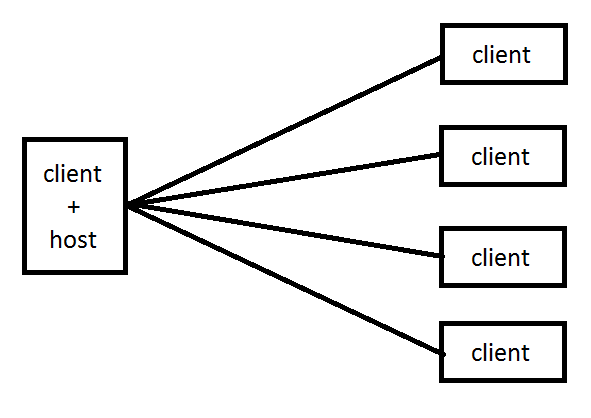
\includegraphics{images/Client_Host.png}
	\caption[Client-Server Modell]{Das Client-Host Modell einfach veranschaulicht}
	\label{pic:Client_Host}
\end{figure}




Bei dieser Variante wird der Serverprozess auf dem selben Gerät ausgeführt, auf dem auch eine Client-Instanz gestartet wurde. Ein Spieler übernimmt also "selbst" das Hosting. Andere Clients haben die Information, welcher Client einen Serverprozess "besitzt" und wie sie sich dorthin verbinden können. 

Vorteile: Die Unabhängigkeit von Hardwareressourcen für Entwickler, dieses "Problem" wird schlichtweg an die Spieler ausgelagert. 

Nachteile: Da der Serverprozess nun ebenfalls auf einem Gerät läuft, auf welches Spieler Zugriff haben gibt es ebenfalls mehr Möglichkeiten des Hackings (Spielmanipulation). Die Entwickler haben keinerlei Einfluss auf die Serverprozesse, welche ein Spieler startet.
\cite{Smed.2002}

"Client-Server":

\begin{figure}
\centering
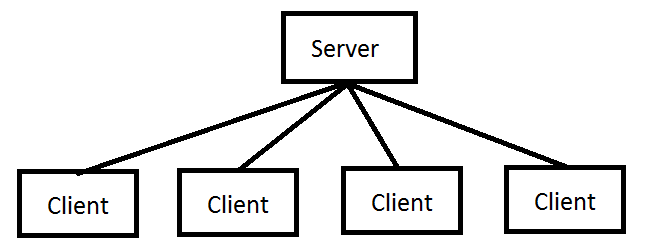
\includegraphics{images/Client_Server.png}
\caption[Client-Server Modell]{Das Client-Server Modell einfach veranschaulicht}
\label{pic:Client_Server}
\end{figure}



Diese Variante trennt Client und Server physikalisch von einander. Serverprozesse werden außerhalb einer Client-Umgebung gestartet und verwaltet. Clients haben einen (oder mehrere) zentrale Zielsysteme, zu welchen sie sich verbinden können.

Vorteile: 

Mehr "Kontrolle" auf Seiten der Entwickler. Hacking ist deutlich erschwert. Die Software-Architektur kann verhindern, dass spielentscheidende Daten nicht in der Hand der Spieler liegen, und somit ein sicheres und faires Spiel gewährleistet werden kann.
\cite{Smed.2002}

Nachteile: 

Die Kosten für Hardware und Bandbreite skalieren mit den Spielerzahlen. Diese Tatsache kann sehr schnell hohe Kosten verursachen. \cite{Deng.2018}

Ein Ausfall des zentralen Servers kann dazu führen, dass ein Großteil der Spielerfahrung nicht mehr spielbar ist. 


\section{Datenspeicherung und Transfer}

Um ein bestmögliches Spielerlebnis zu ermöglichen, sollte innerhalb der Entwicklung von Online Multiplayerspielen darauf geachtet werden, dass spielentscheidende Daten schnellstmöglich zwischen den Clients synchronisiert werden. Wie auch bei anderen Echtzeitsystemen \cite{Wikipedia.2021} kommt es also auch bei der Entwicklung von dieser Art von Software darauf an, Daten zu serialisieren \cite{Wikipedia.2019}. 

Daten unterscheiden sich im Kontext der Online Spielentwicklung grundsätzlich nicht großartig von anderer Software. Typischerweise werden Programmiersprachen wie C\# oder C++ genutzt, um Klassen und Datenstrukturen zu erstellen, welche die eigene Spiellogik abbilden. \cite{Glinka.2008}

Das folgende rudimentäre Klassendiagramm zeigt zwei simple Klassen. Eine Spielerklasse, welche Informationen über den Spieler enthält sowie eine Network Manager Klasse, welche alle Spieler verwaltet.

\begin{figure}
	\centering
	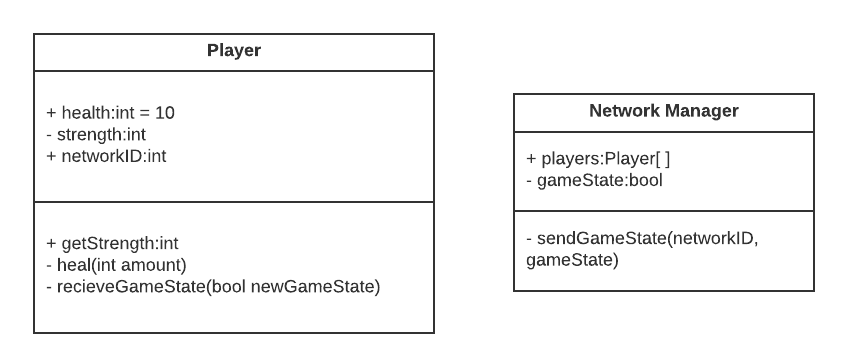
\includegraphics{images/UML_class_Player_NM.png}
	\caption[UML Klassen]{UML Klasse Player und Network Manager}
	\label{pic:UML_class_Player_NM}
\end{figure}

Das Beispiel hat nicht den Anspruch auf Vollständigkeit, soll jedoch illustrieren, auf welche Art und Weise Daten typischerweise innerhalb eines Multiplayer-Kontextes verwaltet werden.

Der Entwickler entscheidet hierbei selbst, welche Informationen in welchem Kontext vorhanden ist. Konkret muss sich ein Entwickler stets die Frage stellen, ob eine Information im Server-Kontext oder im Client-Kontext verwaltet bzw. verarbeitet werden soll.

Serialisierte Daten werden über ein Netzwerk transportiert. Je Nach Art des Hostings erfolgt ein Umweg über eine Server-Instanz, oder direkt zu einem anderen Client. \cite{Smed.2002c}

\section{Kontrolle des Spielflusses}

-> Interest Management


\section{Matchmaking}


// WEITERE IDEEN: Consistency and Responsiveness